% Options for packages loaded elsewhere
\PassOptionsToPackage{unicode}{hyperref}
\PassOptionsToPackage{hyphens}{url}
%
\documentclass[
]{article}
\usepackage{amsmath,amssymb}
\usepackage{lmodern}
\usepackage{iftex}
\ifPDFTeX
  \usepackage[T1]{fontenc}
  \usepackage[utf8]{inputenc}
  \usepackage{textcomp} % provide euro and other symbols
\else % if luatex or xetex
  \usepackage{unicode-math}
  \defaultfontfeatures{Scale=MatchLowercase}
  \defaultfontfeatures[\rmfamily]{Ligatures=TeX,Scale=1}
\fi
% Use upquote if available, for straight quotes in verbatim environments
\IfFileExists{upquote.sty}{\usepackage{upquote}}{}
\IfFileExists{microtype.sty}{% use microtype if available
  \usepackage[]{microtype}
  \UseMicrotypeSet[protrusion]{basicmath} % disable protrusion for tt fonts
}{}
\makeatletter
\@ifundefined{KOMAClassName}{% if non-KOMA class
  \IfFileExists{parskip.sty}{%
    \usepackage{parskip}
  }{% else
    \setlength{\parindent}{0pt}
    \setlength{\parskip}{6pt plus 2pt minus 1pt}}
}{% if KOMA class
  \KOMAoptions{parskip=half}}
\makeatother
\usepackage{xcolor}
\usepackage[margin=1in]{geometry}
\usepackage{color}
\usepackage{fancyvrb}
\newcommand{\VerbBar}{|}
\newcommand{\VERB}{\Verb[commandchars=\\\{\}]}
\DefineVerbatimEnvironment{Highlighting}{Verbatim}{commandchars=\\\{\}}
% Add ',fontsize=\small' for more characters per line
\usepackage{framed}
\definecolor{shadecolor}{RGB}{248,248,248}
\newenvironment{Shaded}{\begin{snugshade}}{\end{snugshade}}
\newcommand{\AlertTok}[1]{\textcolor[rgb]{0.94,0.16,0.16}{#1}}
\newcommand{\AnnotationTok}[1]{\textcolor[rgb]{0.56,0.35,0.01}{\textbf{\textit{#1}}}}
\newcommand{\AttributeTok}[1]{\textcolor[rgb]{0.77,0.63,0.00}{#1}}
\newcommand{\BaseNTok}[1]{\textcolor[rgb]{0.00,0.00,0.81}{#1}}
\newcommand{\BuiltInTok}[1]{#1}
\newcommand{\CharTok}[1]{\textcolor[rgb]{0.31,0.60,0.02}{#1}}
\newcommand{\CommentTok}[1]{\textcolor[rgb]{0.56,0.35,0.01}{\textit{#1}}}
\newcommand{\CommentVarTok}[1]{\textcolor[rgb]{0.56,0.35,0.01}{\textbf{\textit{#1}}}}
\newcommand{\ConstantTok}[1]{\textcolor[rgb]{0.00,0.00,0.00}{#1}}
\newcommand{\ControlFlowTok}[1]{\textcolor[rgb]{0.13,0.29,0.53}{\textbf{#1}}}
\newcommand{\DataTypeTok}[1]{\textcolor[rgb]{0.13,0.29,0.53}{#1}}
\newcommand{\DecValTok}[1]{\textcolor[rgb]{0.00,0.00,0.81}{#1}}
\newcommand{\DocumentationTok}[1]{\textcolor[rgb]{0.56,0.35,0.01}{\textbf{\textit{#1}}}}
\newcommand{\ErrorTok}[1]{\textcolor[rgb]{0.64,0.00,0.00}{\textbf{#1}}}
\newcommand{\ExtensionTok}[1]{#1}
\newcommand{\FloatTok}[1]{\textcolor[rgb]{0.00,0.00,0.81}{#1}}
\newcommand{\FunctionTok}[1]{\textcolor[rgb]{0.00,0.00,0.00}{#1}}
\newcommand{\ImportTok}[1]{#1}
\newcommand{\InformationTok}[1]{\textcolor[rgb]{0.56,0.35,0.01}{\textbf{\textit{#1}}}}
\newcommand{\KeywordTok}[1]{\textcolor[rgb]{0.13,0.29,0.53}{\textbf{#1}}}
\newcommand{\NormalTok}[1]{#1}
\newcommand{\OperatorTok}[1]{\textcolor[rgb]{0.81,0.36,0.00}{\textbf{#1}}}
\newcommand{\OtherTok}[1]{\textcolor[rgb]{0.56,0.35,0.01}{#1}}
\newcommand{\PreprocessorTok}[1]{\textcolor[rgb]{0.56,0.35,0.01}{\textit{#1}}}
\newcommand{\RegionMarkerTok}[1]{#1}
\newcommand{\SpecialCharTok}[1]{\textcolor[rgb]{0.00,0.00,0.00}{#1}}
\newcommand{\SpecialStringTok}[1]{\textcolor[rgb]{0.31,0.60,0.02}{#1}}
\newcommand{\StringTok}[1]{\textcolor[rgb]{0.31,0.60,0.02}{#1}}
\newcommand{\VariableTok}[1]{\textcolor[rgb]{0.00,0.00,0.00}{#1}}
\newcommand{\VerbatimStringTok}[1]{\textcolor[rgb]{0.31,0.60,0.02}{#1}}
\newcommand{\WarningTok}[1]{\textcolor[rgb]{0.56,0.35,0.01}{\textbf{\textit{#1}}}}
\usepackage{graphicx}
\makeatletter
\def\maxwidth{\ifdim\Gin@nat@width>\linewidth\linewidth\else\Gin@nat@width\fi}
\def\maxheight{\ifdim\Gin@nat@height>\textheight\textheight\else\Gin@nat@height\fi}
\makeatother
% Scale images if necessary, so that they will not overflow the page
% margins by default, and it is still possible to overwrite the defaults
% using explicit options in \includegraphics[width, height, ...]{}
\setkeys{Gin}{width=\maxwidth,height=\maxheight,keepaspectratio}
% Set default figure placement to htbp
\makeatletter
\def\fps@figure{htbp}
\makeatother
\setlength{\emergencystretch}{3em} % prevent overfull lines
\providecommand{\tightlist}{%
  \setlength{\itemsep}{0pt}\setlength{\parskip}{0pt}}
\setcounter{secnumdepth}{-\maxdimen} % remove section numbering
\ifLuaTeX
  \usepackage{selnolig}  % disable illegal ligatures
\fi
\IfFileExists{bookmark.sty}{\usepackage{bookmark}}{\usepackage{hyperref}}
\IfFileExists{xurl.sty}{\usepackage{xurl}}{} % add URL line breaks if available
\urlstyle{same} % disable monospaced font for URLs
\hypersetup{
  pdftitle={Project},
  hidelinks,
  pdfcreator={LaTeX via pandoc}}

\title{Project}
\author{}
\date{\vspace{-2.5em}2022-11-28}

\begin{document}
\maketitle

\begin{Shaded}
\begin{Highlighting}[]
\FunctionTok{library}\NormalTok{(tidyverse)}
\end{Highlighting}
\end{Shaded}

\begin{verbatim}
## -- Attaching packages --------------------------------------- tidyverse 1.3.2 --
## v ggplot2 3.4.0      v purrr   0.3.4 
## v tibble  3.1.8      v dplyr   1.0.10
## v tidyr   1.2.0      v stringr 1.4.1 
## v readr   2.1.2      v forcats 0.5.2
\end{verbatim}

\begin{verbatim}
## Warning: 程辑包'ggplot2'是用R版本4.2.2 来建造的
\end{verbatim}

\begin{verbatim}
## -- Conflicts ------------------------------------------ tidyverse_conflicts() --
## x dplyr::filter() masks stats::filter()
## x dplyr::lag()    masks stats::lag()
\end{verbatim}

\begin{Shaded}
\begin{Highlighting}[]
\FunctionTok{library}\NormalTok{(dplyr)}
\FunctionTok{library}\NormalTok{(ggplot2)}
\FunctionTok{library}\NormalTok{(ggcorrplot)}
\end{Highlighting}
\end{Shaded}

\begin{verbatim}
## Warning: 程辑包'ggcorrplot'是用R版本4.2.2 来建造的
\end{verbatim}

\begin{Shaded}
\begin{Highlighting}[]
\FunctionTok{library}\NormalTok{(caret)}
\end{Highlighting}
\end{Shaded}

\begin{verbatim}
## Warning: 程辑包'caret'是用R版本4.2.2 来建造的
\end{verbatim}

\begin{verbatim}
## 载入需要的程辑包:lattice
\end{verbatim}

\begin{verbatim}
## Warning: 程辑包'lattice'是用R版本4.2.2 来建造的
\end{verbatim}

\begin{verbatim}
## 
## 载入程辑包:'caret'
## 
## The following object is masked from 'package:purrr':
## 
##     lift
\end{verbatim}

\begin{Shaded}
\begin{Highlighting}[]
\FunctionTok{library}\NormalTok{(car)}
\end{Highlighting}
\end{Shaded}

\begin{verbatim}
## 载入需要的程辑包:carData
## 
## 载入程辑包:'car'
## 
## The following object is masked from 'package:dplyr':
## 
##     recode
## 
## The following object is masked from 'package:purrr':
## 
##     some
\end{verbatim}

\begin{Shaded}
\begin{Highlighting}[]
\FunctionTok{library}\NormalTok{(glmnet)}
\end{Highlighting}
\end{Shaded}

\begin{verbatim}
## 载入需要的程辑包:Matrix
## 
## 载入程辑包:'Matrix'
## 
## The following objects are masked from 'package:tidyr':
## 
##     expand, pack, unpack
## 
## Loaded glmnet 4.1-4
\end{verbatim}

\begin{Shaded}
\begin{Highlighting}[]
\FunctionTok{library}\NormalTok{(modelr)}
\end{Highlighting}
\end{Shaded}

\hypertarget{description-of-data}{%
\subsection{Description of data}\label{description-of-data}}

\begin{Shaded}
\begin{Highlighting}[]
\NormalTok{bd\_df }\OtherTok{\textless{}{-}}\NormalTok{ readxl}\SpecialCharTok{::}\FunctionTok{read\_excel}\NormalTok{(}\StringTok{"data/body\_density\_data.xlsx"}\NormalTok{)}
\FunctionTok{dim}\NormalTok{(bd\_df)}
\end{Highlighting}
\end{Shaded}

\begin{verbatim}
## [1] 252  17
\end{verbatim}

\begin{Shaded}
\begin{Highlighting}[]
\NormalTok{bd\_df }\OtherTok{\textless{}{-}}\NormalTok{ bd\_df}\SpecialCharTok{\%\textgreater{}\%}
\NormalTok{  dplyr}\SpecialCharTok{::}\FunctionTok{select}\NormalTok{(bodyfat\_brozek, age}\SpecialCharTok{:}\NormalTok{wrist)}\SpecialCharTok{\%\textgreater{}\%}
  \FunctionTok{filter}\NormalTok{(bodyfat\_brozek }\SpecialCharTok{!=} \DecValTok{0}\NormalTok{)}
\end{Highlighting}
\end{Shaded}

We first looked into the content of the dataset. It has 252 observations
across 17 columns. The outcome we selected is bodyfat\_brozek (body fat
calculated by brozek), the other key variables are age, height, weight
and circumference of body part like neck, chest, abdomen, hip, thigh,
knee, ankle, bicep, forearm and wrist.

\hypertarget{plots}{%
\subsection{plots}\label{plots}}

And we use plots to check the distribution of our variables and
relationship between our outcome and each of the variables.

\begin{Shaded}
\begin{Highlighting}[]
\FunctionTok{lapply}\NormalTok{(bd\_df, hist)}
\end{Highlighting}
\end{Shaded}

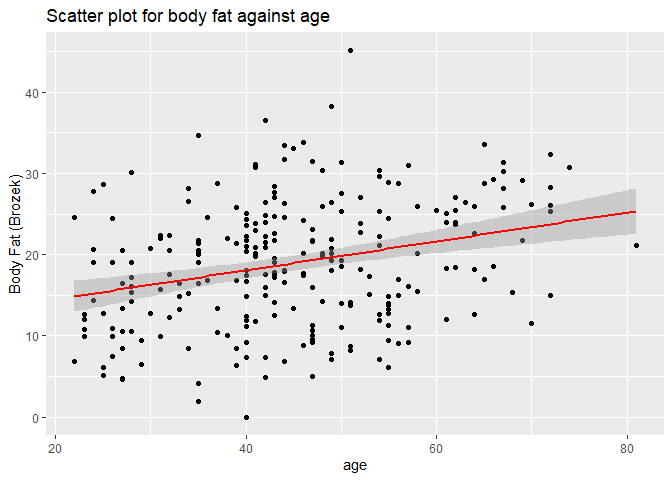
\includegraphics{proj_draft-1-_files/figure-latex/unnamed-chunk-3-1.pdf}
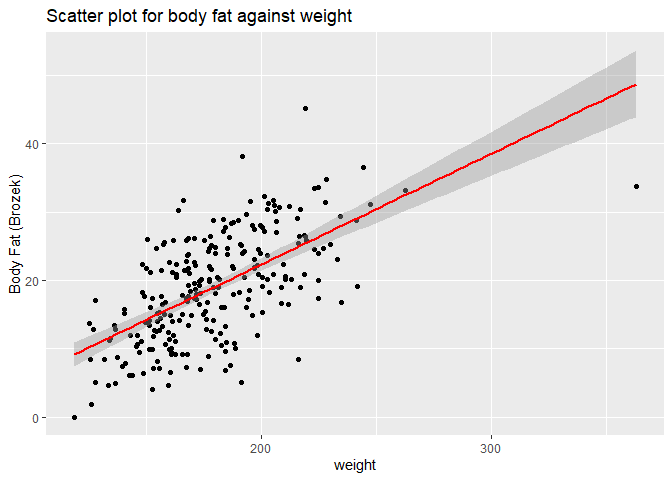
\includegraphics{proj_draft-1-_files/figure-latex/unnamed-chunk-3-2.pdf}
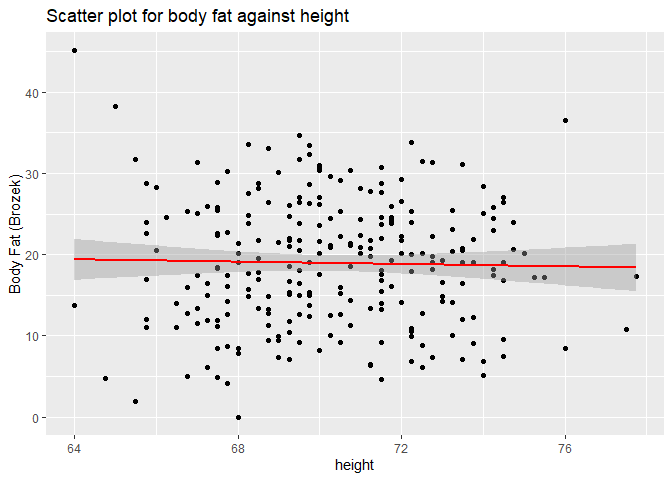
\includegraphics{proj_draft-1-_files/figure-latex/unnamed-chunk-3-3.pdf}
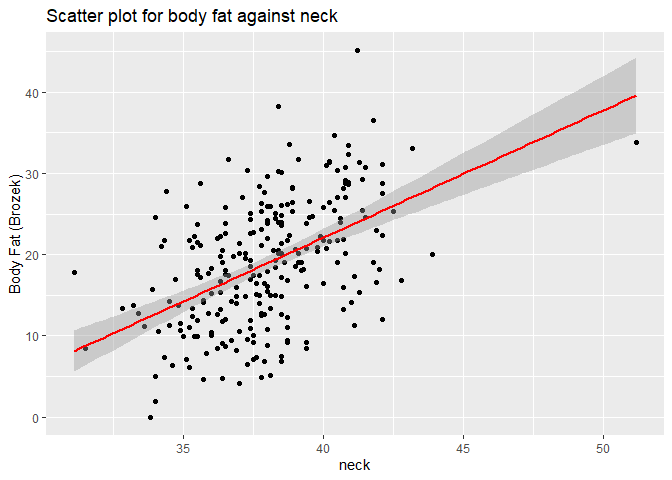
\includegraphics{proj_draft-1-_files/figure-latex/unnamed-chunk-3-4.pdf}
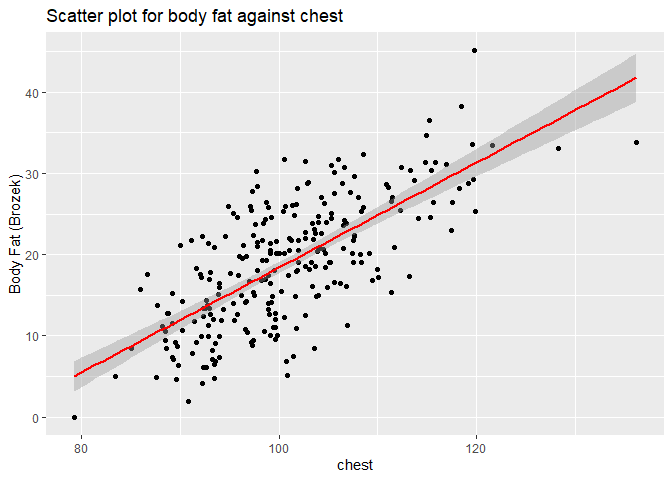
\includegraphics{proj_draft-1-_files/figure-latex/unnamed-chunk-3-5.pdf}
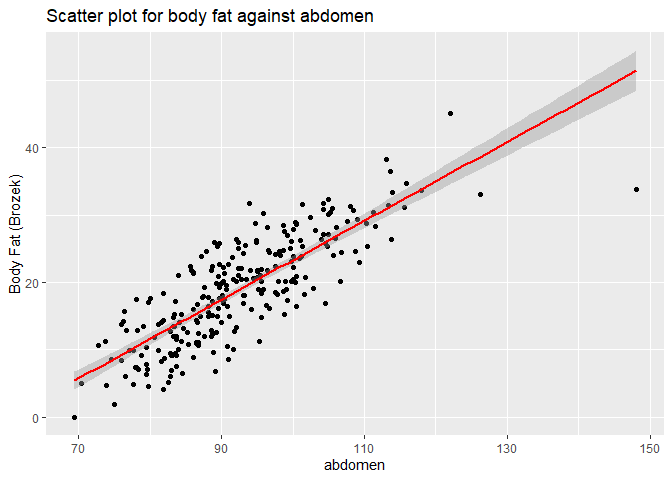
\includegraphics{proj_draft-1-_files/figure-latex/unnamed-chunk-3-6.pdf}
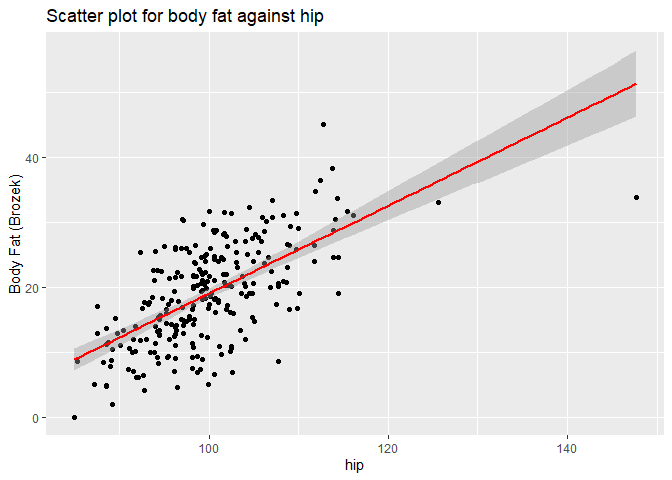
\includegraphics{proj_draft-1-_files/figure-latex/unnamed-chunk-3-7.pdf}
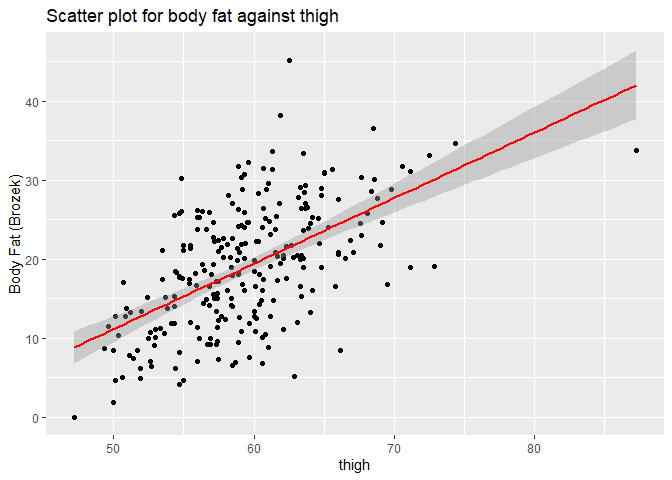
\includegraphics{proj_draft-1-_files/figure-latex/unnamed-chunk-3-8.pdf}
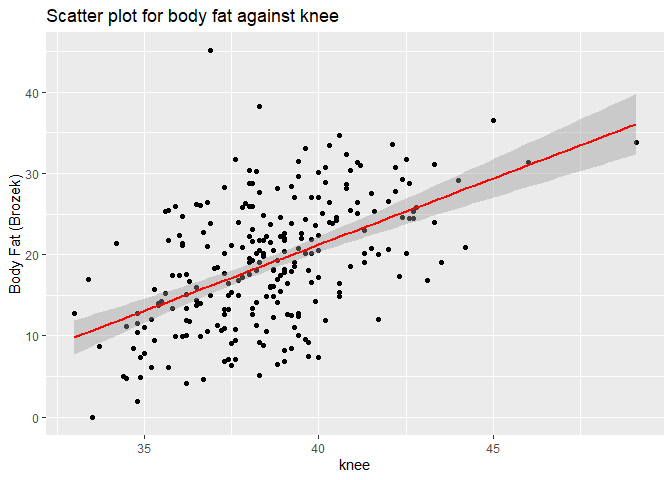
\includegraphics{proj_draft-1-_files/figure-latex/unnamed-chunk-3-9.pdf}
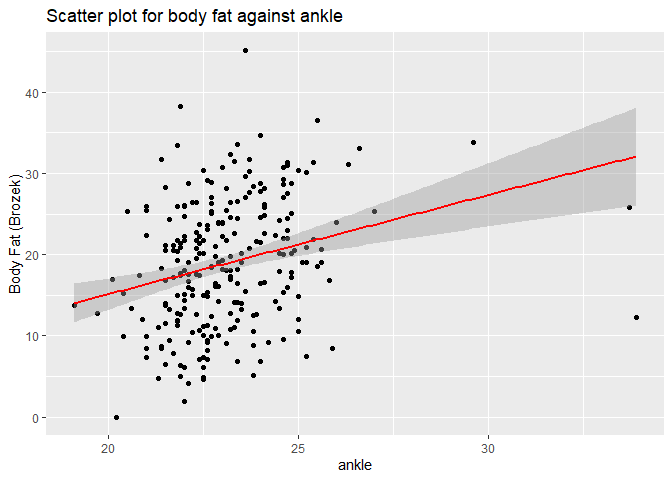
\includegraphics{proj_draft-1-_files/figure-latex/unnamed-chunk-3-10.pdf}
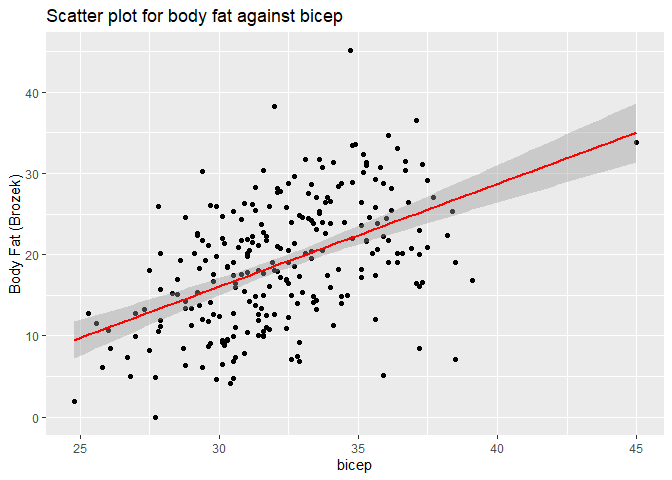
\includegraphics{proj_draft-1-_files/figure-latex/unnamed-chunk-3-11.pdf}
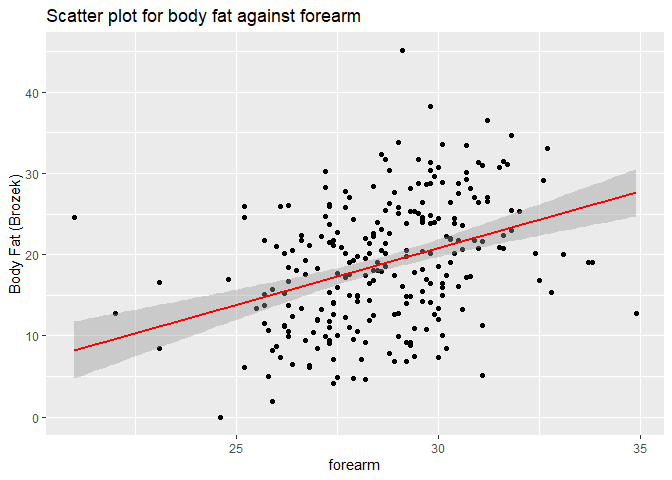
\includegraphics{proj_draft-1-_files/figure-latex/unnamed-chunk-3-12.pdf}
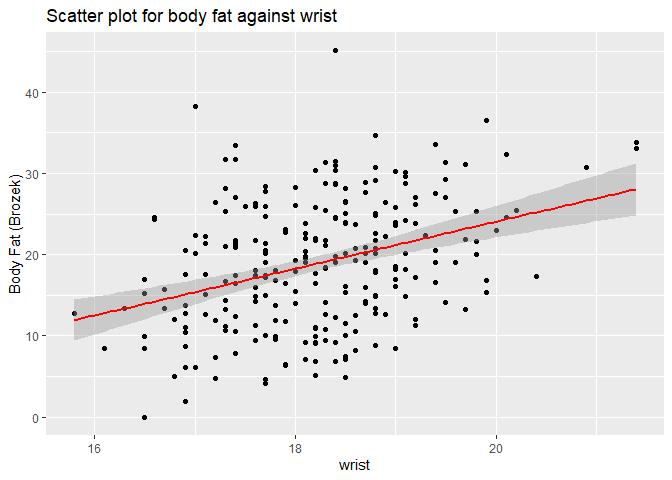
\includegraphics{proj_draft-1-_files/figure-latex/unnamed-chunk-3-13.pdf}
\includegraphics{proj_draft-1-_files/figure-latex/unnamed-chunk-3-14.pdf}

\begin{verbatim}
## $bodyfat_brozek
## $breaks
##  [1]  0  5 10 15 20 25 30 35 40 45 50
## 
## $counts
##  [1]  6 29 48 51 58 37 19  2  0  1
## 
## $density
##  [1] 0.0047808765 0.0231075697 0.0382470120 0.0406374502 0.0462151394
##  [6] 0.0294820717 0.0151394422 0.0015936255 0.0000000000 0.0007968127
## 
## $mids
##  [1]  2.5  7.5 12.5 17.5 22.5 27.5 32.5 37.5 42.5 47.5
## 
## $xname
## [1] "X[[i]]"
## 
## $equidist
## [1] TRUE
## 
## attr(,"class")
## [1] "histogram"
## 
## $age
## $breaks
##  [1] 20 25 30 35 40 45 50 55 60 65 70 75 80 85
## 
## $counts
##  [1] 14 24 25 28 46 38 29 12 17 11  6  0  1
## 
## $density
##  [1] 0.0111553785 0.0191235060 0.0199203187 0.0223107570 0.0366533865
##  [6] 0.0302788845 0.0231075697 0.0095617530 0.0135458167 0.0087649402
## [11] 0.0047808765 0.0000000000 0.0007968127
## 
## $mids
##  [1] 22.5 27.5 32.5 37.5 42.5 47.5 52.5 57.5 62.5 67.5 72.5 77.5 82.5
## 
## $xname
## [1] "X[[i]]"
## 
## $equidist
## [1] TRUE
## 
## attr(,"class")
## [1] "histogram"
## 
## $weight
## $breaks
##  [1] 120 140 160 180 200 220 240 260 280 300 320 340 360 380
## 
## $counts
##  [1] 16 51 77 51 37 13  4  1  0  0  0  0  1
## 
## $density
##  [1] 0.0031872510 0.0101593625 0.0153386454 0.0101593625 0.0073705179
##  [6] 0.0025896414 0.0007968127 0.0001992032 0.0000000000 0.0000000000
## [11] 0.0000000000 0.0000000000 0.0001992032
## 
## $mids
##  [1] 130 150 170 190 210 230 250 270 290 310 330 350 370
## 
## $xname
## [1] "X[[i]]"
## 
## $equidist
## [1] TRUE
## 
## attr(,"class")
## [1] "histogram"
## 
## $height
## $breaks
## [1] 64 66 68 70 72 74 76 78
## 
## $counts
## [1] 14 42 70 58 47 18  2
## 
## $density
## [1] 0.027888446 0.083665339 0.139442231 0.115537849 0.093625498 0.035856574
## [7] 0.003984064
## 
## $mids
## [1] 65 67 69 71 73 75 77
## 
## $xname
## [1] "X[[i]]"
## 
## $equidist
## [1] TRUE
## 
## attr(,"class")
## [1] "histogram"
## 
## $neck
## $breaks
##  [1] 30 32 34 36 38 40 42 44 46 48 50 52
## 
## $counts
##  [1]  2  8 43 81 63 44  9  0  0  0  1
## 
## $density
##  [1] 0.003984064 0.015936255 0.085657371 0.161354582 0.125498008 0.087649402
##  [7] 0.017928287 0.000000000 0.000000000 0.000000000 0.001992032
## 
## $mids
##  [1] 31 33 35 37 39 41 43 45 47 49 51
## 
## $xname
## [1] "X[[i]]"
## 
## $equidist
## [1] TRUE
## 
## attr(,"class")
## [1] "histogram"
## 
## $chest
## $breaks
##  [1]  80  85  90  95 100 105 110 115 120 125 130 135 140
## 
## $counts
##  [1]  1 20 44 64 54 35 15 15  1  1  0  1
## 
## $density
##  [1] 0.0007968127 0.0159362550 0.0350597610 0.0509960159 0.0430278884
##  [6] 0.0278884462 0.0119521912 0.0119521912 0.0007968127 0.0007968127
## [11] 0.0000000000 0.0007968127
## 
## $mids
##  [1]  82.5  87.5  92.5  97.5 102.5 107.5 112.5 117.5 122.5 127.5 132.5 137.5
## 
## $xname
## [1] "X[[i]]"
## 
## $equidist
## [1] TRUE
## 
## attr(,"class")
## [1] "histogram"
## 
## $abdomen
## $breaks
## [1]  70  80  90 100 110 120 130 140 150
## 
## $counts
## [1] 29 84 82 41 12  2  0  1
## 
## $density
## [1] 0.0115537849 0.0334661355 0.0326693227 0.0163346614 0.0047808765
## [6] 0.0007968127 0.0000000000 0.0003984064
## 
## $mids
## [1]  75  85  95 105 115 125 135 145
## 
## $xname
## [1] "X[[i]]"
## 
## $equidist
## [1] TRUE
## 
## attr(,"class")
## [1] "histogram"
## 
## $hip
## $breaks
##  [1]  85  90  95 100 105 110 115 120 125 130 135 140 145 150
## 
## $counts
##  [1] 16 41 84 63 30 13  2  0  1  0  0  0  1
## 
## $density
##  [1] 0.0127490040 0.0326693227 0.0669322709 0.0501992032 0.0239043825
##  [6] 0.0103585657 0.0015936255 0.0000000000 0.0007968127 0.0000000000
## [11] 0.0000000000 0.0000000000 0.0007968127
## 
## $mids
##  [1]  87.5  92.5  97.5 102.5 107.5 112.5 117.5 122.5 127.5 132.5 137.5 142.5
## [13] 147.5
## 
## $xname
## [1] "X[[i]]"
## 
## $equidist
## [1] TRUE
## 
## attr(,"class")
## [1] "histogram"
## 
## $thigh
## $breaks
##  [1] 45 50 55 60 65 70 75 80 85 90
## 
## $counts
## [1]  4 47 96 75 22  6  0  0  1
## 
## $density
## [1] 0.0031872510 0.0374501992 0.0764940239 0.0597609562 0.0175298805
## [6] 0.0047808765 0.0000000000 0.0000000000 0.0007968127
## 
## $mids
## [1] 47.5 52.5 57.5 62.5 67.5 72.5 77.5 82.5 87.5
## 
## $xname
## [1] "X[[i]]"
## 
## $equidist
## [1] TRUE
## 
## attr(,"class")
## [1] "histogram"
## 
## $knee
## $breaks
##  [1] 32 34 36 38 40 42 44 46 48 50
## 
## $counts
## [1]  3 32 64 95 34 19  3  0  1
## 
## $density
## [1] 0.005976096 0.063745020 0.127490040 0.189243028 0.067729084 0.037848606
## [7] 0.005976096 0.000000000 0.001992032
## 
## $mids
## [1] 33 35 37 39 41 43 45 47 49
## 
## $xname
## [1] "X[[i]]"
## 
## $equidist
## [1] TRUE
## 
## attr(,"class")
## [1] "histogram"
## 
## $ankle
## $breaks
## [1] 18 20 22 24 26 28 30 32 34
## 
## $counts
## [1]   2  63 128  52   3   1   0   2
## 
## $density
## [1] 0.003984064 0.125498008 0.254980080 0.103585657 0.005976096 0.001992032
## [7] 0.000000000 0.003984064
## 
## $mids
## [1] 19 21 23 25 27 29 31 33
## 
## $xname
## [1] "X[[i]]"
## 
## $equidist
## [1] TRUE
## 
## attr(,"class")
## [1] "histogram"
## 
## $bicep
## $breaks
##  [1] 24 26 28 30 32 34 36 38 40 42 44 46
## 
## $counts
##  [1]  5 15 35 70 59 37 24  5  0  0  1
## 
## $density
##  [1] 0.009960159 0.029880478 0.069721116 0.139442231 0.117529880 0.073705179
##  [7] 0.047808765 0.009960159 0.000000000 0.000000000 0.001992032
## 
## $mids
##  [1] 25 27 29 31 33 35 37 39 41 43 45
## 
## $xname
## [1] "X[[i]]"
## 
## $equidist
## [1] TRUE
## 
## attr(,"class")
## [1] "histogram"
## 
## $forearm
## $breaks
## [1] 20 22 24 26 28 30 32 34 36
## 
## $counts
## [1]  2  2 16 77 93 52  8  1
## 
## $density
## [1] 0.003984064 0.003984064 0.031872510 0.153386454 0.185258964 0.103585657
## [7] 0.015936255 0.001992032
## 
## $mids
## [1] 21 23 25 27 29 31 33 35
## 
## $xname
## [1] "X[[i]]"
## 
## $equidist
## [1] TRUE
## 
## attr(,"class")
## [1] "histogram"
## 
## $wrist
## $breaks
##  [1] 15.5 16.0 16.5 17.0 17.5 18.0 18.5 19.0 19.5 20.0 20.5 21.0 21.5
## 
## $counts
##  [1]  1  6 19 32 43 63 45 23 12  4  1  2
## 
## $density
##  [1] 0.007968127 0.047808765 0.151394422 0.254980080 0.342629482 0.501992032
##  [7] 0.358565737 0.183266932 0.095617530 0.031872510 0.007968127 0.015936255
## 
## $mids
##  [1] 15.75 16.25 16.75 17.25 17.75 18.25 18.75 19.25 19.75 20.25 20.75 21.25
## 
## $xname
## [1] "X[[i]]"
## 
## $equidist
## [1] TRUE
## 
## attr(,"class")
## [1] "histogram"
\end{verbatim}

\begin{Shaded}
\begin{Highlighting}[]
\FunctionTok{par}\NormalTok{(}\AttributeTok{mfrow =} \FunctionTok{c}\NormalTok{(}\DecValTok{2}\NormalTok{,}\DecValTok{2}\NormalTok{))}
\FunctionTok{lapply}\NormalTok{(}\FunctionTok{colnames}\NormalTok{(bd\_df)[}\DecValTok{2}\SpecialCharTok{:}\FunctionTok{length}\NormalTok{(}\FunctionTok{colnames}\NormalTok{(bd\_df))], }\ControlFlowTok{function}\NormalTok{(nm)\{}
  \FunctionTok{ggplot}\NormalTok{(bd\_df) }\SpecialCharTok{+}
    \FunctionTok{geom\_point}\NormalTok{(}\FunctionTok{aes\_string}\NormalTok{(}\AttributeTok{y =}\FunctionTok{colnames}\NormalTok{(bd\_df)[}\DecValTok{1}\NormalTok{],}
\NormalTok{                          nm))}
\NormalTok{\})}
\end{Highlighting}
\end{Shaded}

\begin{verbatim}
## Warning: `aes_string()` was deprecated in ggplot2 3.0.0.
## i Please use tidy evaluation ideoms with `aes()`
\end{verbatim}

\begin{verbatim}
## [[1]]
\end{verbatim}

\includegraphics{proj_draft-1-_files/figure-latex/unnamed-chunk-4-1.pdf}

\begin{verbatim}
## 
## [[2]]
\end{verbatim}

\includegraphics{proj_draft-1-_files/figure-latex/unnamed-chunk-4-2.pdf}

\begin{verbatim}
## 
## [[3]]
\end{verbatim}

\includegraphics{proj_draft-1-_files/figure-latex/unnamed-chunk-4-3.pdf}

\begin{verbatim}
## 
## [[4]]
\end{verbatim}

\includegraphics{proj_draft-1-_files/figure-latex/unnamed-chunk-4-4.pdf}

\begin{verbatim}
## 
## [[5]]
\end{verbatim}

\includegraphics{proj_draft-1-_files/figure-latex/unnamed-chunk-4-5.pdf}

\begin{verbatim}
## 
## [[6]]
\end{verbatim}

\includegraphics{proj_draft-1-_files/figure-latex/unnamed-chunk-4-6.pdf}

\begin{verbatim}
## 
## [[7]]
\end{verbatim}

\includegraphics{proj_draft-1-_files/figure-latex/unnamed-chunk-4-7.pdf}

\begin{verbatim}
## 
## [[8]]
\end{verbatim}

\includegraphics{proj_draft-1-_files/figure-latex/unnamed-chunk-4-8.pdf}

\begin{verbatim}
## 
## [[9]]
\end{verbatim}

\includegraphics{proj_draft-1-_files/figure-latex/unnamed-chunk-4-9.pdf}

\begin{verbatim}
## 
## [[10]]
\end{verbatim}

\includegraphics{proj_draft-1-_files/figure-latex/unnamed-chunk-4-10.pdf}

\begin{verbatim}
## 
## [[11]]
\end{verbatim}

\includegraphics{proj_draft-1-_files/figure-latex/unnamed-chunk-4-11.pdf}

\begin{verbatim}
## 
## [[12]]
\end{verbatim}

\includegraphics{proj_draft-1-_files/figure-latex/unnamed-chunk-4-12.pdf}

\begin{verbatim}
## 
## [[13]]
\end{verbatim}

\includegraphics{proj_draft-1-_files/figure-latex/unnamed-chunk-4-13.pdf}

From the plots, it seems that all data are symmetrically distributed. We
also saw that there is no obvious relation ship between height and body
fat.

\begin{Shaded}
\begin{Highlighting}[]
\FunctionTok{set.seed}\NormalTok{(}\DecValTok{1}\NormalTok{)}
\NormalTok{sub}\OtherTok{\textless{}{-}}\FunctionTok{sample}\NormalTok{(}\FunctionTok{nrow}\NormalTok{(bd\_df),}\FunctionTok{round}\NormalTok{(}\FunctionTok{nrow}\NormalTok{(bd\_df)}\SpecialCharTok{*}\FloatTok{0.8}\NormalTok{))}
\NormalTok{data\_train}\OtherTok{\textless{}{-}}\NormalTok{bd\_df[sub,]}
\NormalTok{data\_test}\OtherTok{\textless{}{-}}\NormalTok{bd\_df[}\SpecialCharTok{{-}}\NormalTok{sub,]}
\NormalTok{X.test }\OtherTok{=} \FunctionTok{as.matrix}\NormalTok{(data\_test[,}\SpecialCharTok{{-}}\DecValTok{1}\NormalTok{]) }
\NormalTok{Y.test }\OtherTok{=} \FunctionTok{as.matrix}\NormalTok{(data\_test[,}\DecValTok{1}\NormalTok{])}
\NormalTok{X.train }\OtherTok{=} \FunctionTok{as.matrix}\NormalTok{(data\_train[,}\SpecialCharTok{{-}}\DecValTok{1}\NormalTok{]) }
\NormalTok{Y.train }\OtherTok{=} \FunctionTok{as.matrix}\NormalTok{(data\_train[,}\DecValTok{1}\NormalTok{])}
\end{Highlighting}
\end{Shaded}

\hypertarget{use-stepwise-methods}{%
\subsection{Use stepwise methods}\label{use-stepwise-methods}}

\begin{Shaded}
\begin{Highlighting}[]
\NormalTok{full\_fit }\OtherTok{=} \FunctionTok{lm}\NormalTok{(bodyfat\_brozek }\SpecialCharTok{\textasciitilde{}}\NormalTok{ age }\SpecialCharTok{+}\NormalTok{ height }\SpecialCharTok{+}\NormalTok{weight }\SpecialCharTok{+}\NormalTok{ neck }\SpecialCharTok{+}\NormalTok{ chest }\SpecialCharTok{+}\NormalTok{ abdomen }\SpecialCharTok{+}\NormalTok{ hip }\SpecialCharTok{+}\NormalTok{ thigh }\SpecialCharTok{+}\NormalTok{ knee }\SpecialCharTok{+}\NormalTok{ ankle }\SpecialCharTok{+}\NormalTok{ bicep }\SpecialCharTok{+}\NormalTok{forearm }\SpecialCharTok{+}\NormalTok{ wrist, }\AttributeTok{data =}\NormalTok{ data\_train)}
\NormalTok{Step\_model\_1 }\OtherTok{=} \FunctionTok{step}\NormalTok{(full\_fit, }\AttributeTok{direction =} \StringTok{"backward"}\NormalTok{, }\AttributeTok{trace =} \DecValTok{0}\NormalTok{)}
\FunctionTok{summary}\NormalTok{(Step\_model\_1)}
\end{Highlighting}
\end{Shaded}

\begin{verbatim}
## 
## Call:
## lm(formula = bodyfat_brozek ~ age + neck + chest + abdomen + 
##     hip + thigh + forearm + wrist, data = data_train)
## 
## Residuals:
##     Min      1Q  Median      3Q     Max 
## -8.4727 -2.7587 -0.1712  2.9613  9.7228 
## 
## Coefficients:
##             Estimate Std. Error t value Pr(>|t|)    
## (Intercept)  8.37001    6.90530   1.212  0.22696    
## age          0.06877    0.03061   2.247  0.02580 *  
## neck        -0.43484    0.21659  -2.008  0.04608 *  
## chest       -0.16575    0.09418  -1.760  0.08001 .  
## abdomen      0.91764    0.08543  10.741  < 2e-16 ***
## hip         -0.35018    0.11963  -2.927  0.00383 ** 
## thigh        0.23851    0.12836   1.858  0.06467 .  
## forearm      0.69146    0.22744   3.040  0.00269 ** 
## wrist       -2.38737    0.49371  -4.836 2.72e-06 ***
## ---
## Signif. codes:  0 '***' 0.001 '**' 0.01 '*' 0.05 '.' 0.1 ' ' 1
## 
## Residual standard error: 3.865 on 192 degrees of freedom
## Multiple R-squared:  0.7565, Adjusted R-squared:  0.7463 
## F-statistic: 74.55 on 8 and 192 DF,  p-value: < 2.2e-16
\end{verbatim}

\begin{Shaded}
\begin{Highlighting}[]
\FunctionTok{vif}\NormalTok{(Step\_model\_1)}
\end{Highlighting}
\end{Shaded}

\begin{verbatim}
##       age      neck     chest   abdomen       hip     thigh   forearm     wrist 
##  1.900663  3.725082  8.143448 11.570329 10.199697  6.401295  2.569941  2.663161
\end{verbatim}

\begin{Shaded}
\begin{Highlighting}[]
\FunctionTok{plot}\NormalTok{(Step\_model\_1)}
\end{Highlighting}
\end{Shaded}

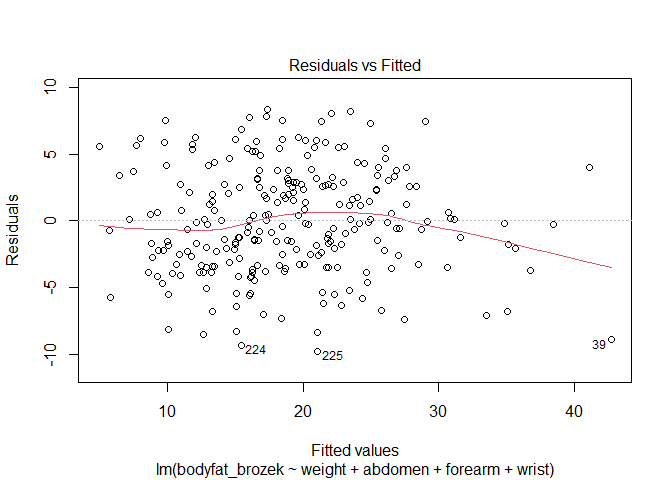
\includegraphics{proj_draft-1-_files/figure-latex/unnamed-chunk-6-1.pdf}
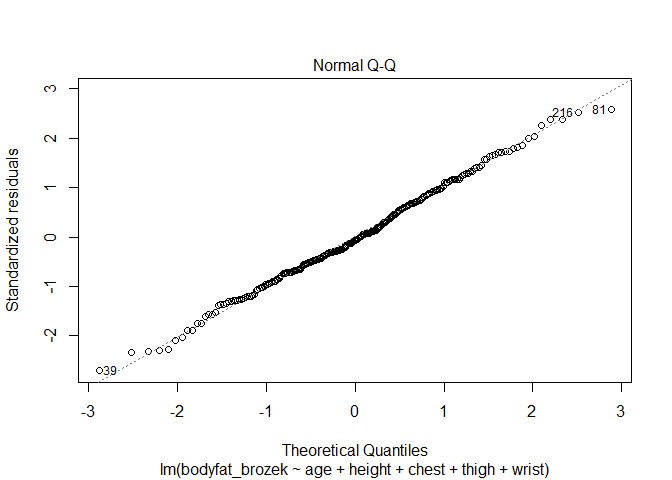
\includegraphics{proj_draft-1-_files/figure-latex/unnamed-chunk-6-2.pdf}
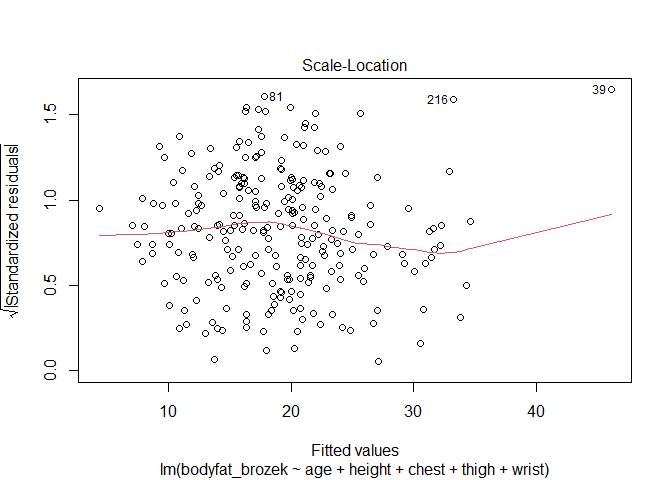
\includegraphics{proj_draft-1-_files/figure-latex/unnamed-chunk-6-3.pdf}
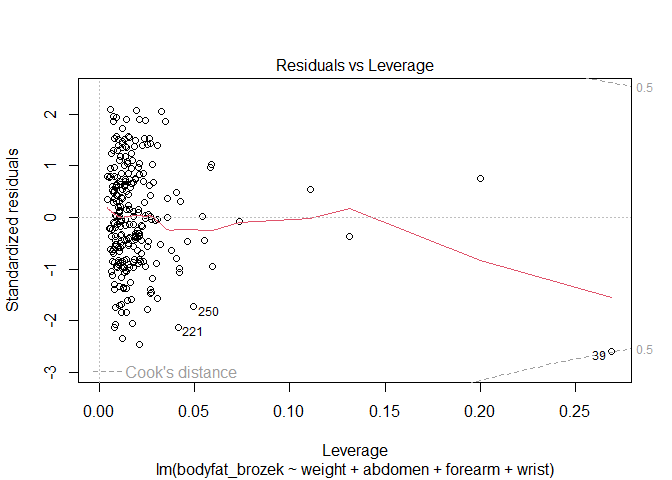
\includegraphics{proj_draft-1-_files/figure-latex/unnamed-chunk-6-4.pdf}

\begin{Shaded}
\begin{Highlighting}[]
\NormalTok{RMSE\_Step }\OtherTok{\textless{}{-}} \FunctionTok{rmse}\NormalTok{(Step\_model\_1,}\AttributeTok{data =}\NormalTok{ data\_test)}
\NormalTok{RMSE\_Step}
\end{Highlighting}
\end{Shaded}

\begin{verbatim}
## [1] 4.687117
\end{verbatim}

Although circumference of hip is included in the stepwise model, it is
not significant. We then calculated VIF in our stepwise model and found
that the VIF of hip is \textgreater10. So we doubted that whether it can
be included in a model.

\begin{Shaded}
\begin{Highlighting}[]
\NormalTok{model2 }\OtherTok{\textless{}{-}} \FunctionTok{lm}\NormalTok{(bodyfat\_brozek }\SpecialCharTok{\textasciitilde{}}\NormalTok{ age  }\SpecialCharTok{+}\NormalTok{weight }\SpecialCharTok{+}\NormalTok{ neck }\SpecialCharTok{+}\NormalTok{ abdomen  }\SpecialCharTok{+}\NormalTok{ thigh  }\SpecialCharTok{+}\NormalTok{forearm }\SpecialCharTok{+}\NormalTok{ wrist, }\AttributeTok{data =}\NormalTok{ data\_train)}
\FunctionTok{anova}\NormalTok{(Step\_model\_1,model2)}
\end{Highlighting}
\end{Shaded}

\begin{verbatim}
## Analysis of Variance Table
## 
## Model 1: bodyfat_brozek ~ age + neck + chest + abdomen + hip + thigh + 
##     forearm + wrist
## Model 2: bodyfat_brozek ~ age + weight + neck + abdomen + thigh + forearm + 
##     wrist
##   Res.Df    RSS Df Sum of Sq      F  Pr(>F)  
## 1    192 2867.5                              
## 2    193 2915.2 -1   -47.756 3.1977 0.07532 .
## ---
## Signif. codes:  0 '***' 0.001 '**' 0.01 '*' 0.05 '.' 0.1 ' ' 1
\end{verbatim}

\begin{Shaded}
\begin{Highlighting}[]
\FunctionTok{summary}\NormalTok{(model2)}
\end{Highlighting}
\end{Shaded}

\begin{verbatim}
## 
## Call:
## lm(formula = bodyfat_brozek ~ age + weight + neck + abdomen + 
##     thigh + forearm + wrist, data = data_train)
## 
## Residuals:
##     Min      1Q  Median      3Q     Max 
## -8.6730 -2.6112 -0.1597  2.4925  8.6731 
## 
## Coefficients:
##              Estimate Std. Error t value Pr(>|t|)    
## (Intercept) -24.29952    9.16755  -2.651 0.008702 ** 
## age           0.06250    0.03145   1.987 0.048287 *  
## weight       -0.10653    0.03503  -3.041 0.002685 ** 
## neck         -0.30666    0.22091  -1.388 0.166683    
## abdomen       0.83136    0.06926  12.003  < 2e-16 ***
## thigh         0.20293    0.11774   1.724 0.086392 .  
## forearm       0.66901    0.21950   3.048 0.002628 ** 
## wrist        -2.04676    0.52904  -3.869 0.000149 ***
## ---
## Signif. codes:  0 '***' 0.001 '**' 0.01 '*' 0.05 '.' 0.1 ' ' 1
## 
## Residual standard error: 3.887 on 193 degrees of freedom
## Multiple R-squared:  0.7524, Adjusted R-squared:  0.7434 
## F-statistic: 83.79 on 7 and 193 DF,  p-value: < 2.2e-16
\end{verbatim}

\begin{Shaded}
\begin{Highlighting}[]
\NormalTok{RMSE\_2 }\OtherTok{\textless{}{-}} \FunctionTok{rmse}\NormalTok{(model2,}\AttributeTok{data =}\NormalTok{ data\_test)}
\NormalTok{RMSE\_2}
\end{Highlighting}
\end{Shaded}

\begin{verbatim}
## [1] 4.429224
\end{verbatim}

We performed ANOVA on these two models, p-value is greater than 0.05.
The ANOVA test indicates that the model not include hip circumference
may be better. This model also has a lower BIC. However, it's AIC is
larger than the stepwise model and adj R-squared is also a little bit
smaller than the stepwise model. Therefore, we can't decided our final
model yet.

\begin{Shaded}
\begin{Highlighting}[]
\NormalTok{mat }\OtherTok{=} \FunctionTok{as.matrix}\NormalTok{(data\_train)}
\NormalTok{leaps}\SpecialCharTok{::}\FunctionTok{leaps}\NormalTok{(}\AttributeTok{x =}\NormalTok{ mat[,}\SpecialCharTok{{-}}\DecValTok{1}\NormalTok{], }\AttributeTok{y =}\NormalTok{ mat[,}\DecValTok{1}\NormalTok{], }\AttributeTok{nbest =} \DecValTok{1}\NormalTok{, }\AttributeTok{method =} \StringTok{"Cp"}\NormalTok{)}
\end{Highlighting}
\end{Shaded}

\begin{verbatim}
## $which
##        1     2     3     4     5    6     7     8     9     A     B     C     D
## 1  FALSE FALSE FALSE FALSE FALSE TRUE FALSE FALSE FALSE FALSE FALSE FALSE FALSE
## 2  FALSE  TRUE FALSE FALSE FALSE TRUE FALSE FALSE FALSE FALSE FALSE FALSE FALSE
## 3  FALSE  TRUE FALSE FALSE FALSE TRUE FALSE FALSE FALSE FALSE FALSE FALSE  TRUE
## 4  FALSE  TRUE FALSE FALSE FALSE TRUE FALSE FALSE FALSE FALSE FALSE  TRUE  TRUE
## 5  FALSE  TRUE FALSE FALSE  TRUE TRUE FALSE FALSE FALSE FALSE FALSE  TRUE  TRUE
## 6   TRUE  TRUE FALSE FALSE FALSE TRUE FALSE  TRUE FALSE FALSE FALSE  TRUE  TRUE
## 7   TRUE FALSE FALSE  TRUE FALSE TRUE  TRUE  TRUE FALSE FALSE FALSE  TRUE  TRUE
## 8   TRUE FALSE FALSE  TRUE  TRUE TRUE  TRUE  TRUE FALSE FALSE FALSE  TRUE  TRUE
## 9   TRUE FALSE FALSE  TRUE  TRUE TRUE  TRUE  TRUE  TRUE FALSE FALSE  TRUE  TRUE
## 10  TRUE  TRUE FALSE  TRUE  TRUE TRUE  TRUE  TRUE  TRUE FALSE FALSE  TRUE  TRUE
## 11  TRUE  TRUE FALSE  TRUE  TRUE TRUE  TRUE  TRUE  TRUE FALSE  TRUE  TRUE  TRUE
## 12  TRUE  TRUE FALSE  TRUE  TRUE TRUE  TRUE  TRUE  TRUE  TRUE  TRUE  TRUE  TRUE
## 13  TRUE  TRUE  TRUE  TRUE  TRUE TRUE  TRUE  TRUE  TRUE  TRUE  TRUE  TRUE  TRUE
## 
## $label
##  [1] "(Intercept)" "1"           "2"           "3"           "4"          
##  [6] "5"           "6"           "7"           "8"           "9"          
## [11] "A"           "B"           "C"           "D"          
## 
## $size
##  [1]  2  3  4  5  6  7  8  9 10 11 12 13 14
## 
## $Cp
##  [1] 67.593447 26.429086 15.256941  8.953374  8.759300  8.133340  8.105090
##  [8]  7.039263  7.283463  8.735947 10.389678 12.094124 14.000000
\end{verbatim}

\begin{Shaded}
\begin{Highlighting}[]
\NormalTok{leaps}\SpecialCharTok{::}\FunctionTok{leaps}\NormalTok{(}\AttributeTok{x =}\NormalTok{ mat[,}\SpecialCharTok{{-}}\DecValTok{1}\NormalTok{], }\AttributeTok{y =}\NormalTok{ mat[,}\DecValTok{1}\NormalTok{], }\AttributeTok{nbest =} \DecValTok{1}\NormalTok{, }\AttributeTok{method =} \StringTok{"adjr2"}\NormalTok{)}
\end{Highlighting}
\end{Shaded}

\begin{verbatim}
## $which
##        1     2     3     4     5    6     7     8     9     A     B     C     D
## 1  FALSE FALSE FALSE FALSE FALSE TRUE FALSE FALSE FALSE FALSE FALSE FALSE FALSE
## 2  FALSE  TRUE FALSE FALSE FALSE TRUE FALSE FALSE FALSE FALSE FALSE FALSE FALSE
## 3  FALSE  TRUE FALSE FALSE FALSE TRUE FALSE FALSE FALSE FALSE FALSE FALSE  TRUE
## 4  FALSE  TRUE FALSE FALSE FALSE TRUE FALSE FALSE FALSE FALSE FALSE  TRUE  TRUE
## 5  FALSE  TRUE FALSE FALSE  TRUE TRUE FALSE FALSE FALSE FALSE FALSE  TRUE  TRUE
## 6   TRUE  TRUE FALSE FALSE FALSE TRUE FALSE  TRUE FALSE FALSE FALSE  TRUE  TRUE
## 7   TRUE FALSE FALSE  TRUE FALSE TRUE  TRUE  TRUE FALSE FALSE FALSE  TRUE  TRUE
## 8   TRUE FALSE FALSE  TRUE  TRUE TRUE  TRUE  TRUE FALSE FALSE FALSE  TRUE  TRUE
## 9   TRUE FALSE FALSE  TRUE  TRUE TRUE  TRUE  TRUE  TRUE FALSE FALSE  TRUE  TRUE
## 10  TRUE  TRUE FALSE  TRUE  TRUE TRUE  TRUE  TRUE  TRUE FALSE FALSE  TRUE  TRUE
## 11  TRUE  TRUE FALSE  TRUE  TRUE TRUE  TRUE  TRUE  TRUE FALSE  TRUE  TRUE  TRUE
## 12  TRUE  TRUE FALSE  TRUE  TRUE TRUE  TRUE  TRUE  TRUE  TRUE  TRUE  TRUE  TRUE
## 13  TRUE  TRUE  TRUE  TRUE  TRUE TRUE  TRUE  TRUE  TRUE  TRUE  TRUE  TRUE  TRUE
## 
## $label
##  [1] "(Intercept)" "1"           "2"           "3"           "4"          
##  [6] "5"           "6"           "7"           "8"           "9"          
## [11] "A"           "B"           "C"           "D"          
## 
## $size
##  [1]  2  3  4  5  6  7  8  9 10 11 12 13 14
## 
## $adjr2
##  [1] 0.6592385 0.7133883 0.7290696 0.7385449 0.7400877 0.7422170 0.7435747
##  [8] 0.7463315 0.7473593 0.7467682 0.7458979 0.7449492 0.7437142
\end{verbatim}

If we choose predictors based on Cp, The Cp is the smallest when the
predictors are age, neck,chest, abdomen,hip, thigh, forearm and wrist.
If we choose predictors based on adjust R-squared, the predictors are
the same.

fitted model based on above Criterion

\begin{Shaded}
\begin{Highlighting}[]
\NormalTok{model3 }\OtherTok{\textless{}{-}} \FunctionTok{lm}\NormalTok{(bodyfat\_brozek }\SpecialCharTok{\textasciitilde{}}\NormalTok{ age }\SpecialCharTok{+}\NormalTok{  neck }\SpecialCharTok{+}\NormalTok{ chest }\SpecialCharTok{+}\NormalTok{ abdomen }\SpecialCharTok{+}\NormalTok{ hip }\SpecialCharTok{+}\NormalTok{ thigh  }\SpecialCharTok{+}\NormalTok{forearm }\SpecialCharTok{+}\NormalTok{ wrist, }\AttributeTok{data =}\NormalTok{ data\_train)}
\FunctionTok{summary}\NormalTok{(model3)}
\end{Highlighting}
\end{Shaded}

\begin{verbatim}
## 
## Call:
## lm(formula = bodyfat_brozek ~ age + neck + chest + abdomen + 
##     hip + thigh + forearm + wrist, data = data_train)
## 
## Residuals:
##     Min      1Q  Median      3Q     Max 
## -8.4727 -2.7587 -0.1712  2.9613  9.7228 
## 
## Coefficients:
##             Estimate Std. Error t value Pr(>|t|)    
## (Intercept)  8.37001    6.90530   1.212  0.22696    
## age          0.06877    0.03061   2.247  0.02580 *  
## neck        -0.43484    0.21659  -2.008  0.04608 *  
## chest       -0.16575    0.09418  -1.760  0.08001 .  
## abdomen      0.91764    0.08543  10.741  < 2e-16 ***
## hip         -0.35018    0.11963  -2.927  0.00383 ** 
## thigh        0.23851    0.12836   1.858  0.06467 .  
## forearm      0.69146    0.22744   3.040  0.00269 ** 
## wrist       -2.38737    0.49371  -4.836 2.72e-06 ***
## ---
## Signif. codes:  0 '***' 0.001 '**' 0.01 '*' 0.05 '.' 0.1 ' ' 1
## 
## Residual standard error: 3.865 on 192 degrees of freedom
## Multiple R-squared:  0.7565, Adjusted R-squared:  0.7463 
## F-statistic: 74.55 on 8 and 192 DF,  p-value: < 2.2e-16
\end{verbatim}

\begin{Shaded}
\begin{Highlighting}[]
\NormalTok{RMSE\_3 }\OtherTok{\textless{}{-}} \FunctionTok{rmse}\NormalTok{(model3,}\AttributeTok{data =}\NormalTok{ data\_test)}
\NormalTok{RMSE\_3}
\end{Highlighting}
\end{Shaded}

\begin{verbatim}
## [1] 4.687117
\end{verbatim}

\hypertarget{lasso}{%
\subsection{LASSO}\label{lasso}}

We also want to use LASSO to generate a reasonable model. First, we want
to choose the best lambda. So we conducted a cross validation. The cross
validation's result shows that the best lambda is 0.04,which is small.
This indicates that we may include many variables in our model if we
using LASSO. So we fit a model with LASSO Regression.

\begin{Shaded}
\begin{Highlighting}[]
\FunctionTok{set.seed}\NormalTok{(}\DecValTok{123}\NormalTok{)}
\NormalTok{lambda\_seq }\OtherTok{\textless{}{-}} \DecValTok{10}\SpecialCharTok{\^{}}\FunctionTok{seq}\NormalTok{(}\SpecialCharTok{{-}}\DecValTok{3}\NormalTok{, }\DecValTok{0}\NormalTok{, }\AttributeTok{by =}\NormalTok{ .}\DecValTok{1}\NormalTok{)}
\NormalTok{cv\_object }\OtherTok{\textless{}{-}} \FunctionTok{cv.glmnet}\NormalTok{(}\FunctionTok{as.matrix}\NormalTok{(data\_train[,}\SpecialCharTok{{-}}\DecValTok{1}\NormalTok{]), data\_train}\SpecialCharTok{$}\NormalTok{bodyfat\_brozek, }\AttributeTok{lambda =}\NormalTok{ lambda\_seq, }
\AttributeTok{nfolds =} \DecValTok{5}\NormalTok{)}
\NormalTok{cv\_object}
\end{Highlighting}
\end{Shaded}

\begin{verbatim}
## 
## Call:  cv.glmnet(x = as.matrix(data_train[, -1]), y = data_train$bodyfat_brozek,      lambda = lambda_seq, nfolds = 5) 
## 
## Measure: Mean-Squared Error 
## 
##     Lambda Index Measure    SE Nonzero
## min 0.0251    17   17.50 1.887      12
## 1se 0.5012     4   18.89 1.377       4
\end{verbatim}

\begin{Shaded}
\begin{Highlighting}[]
\FunctionTok{tibble}\NormalTok{(}\AttributeTok{lambda =}\NormalTok{ cv\_object}\SpecialCharTok{$}\NormalTok{lambda,}
\AttributeTok{mean\_cv\_error =}\NormalTok{ cv\_object}\SpecialCharTok{$}\NormalTok{cvm) }\SpecialCharTok{\%\textgreater{}\%}
\FunctionTok{ggplot}\NormalTok{(}\FunctionTok{aes}\NormalTok{(}\AttributeTok{x =}\NormalTok{ lambda, }\AttributeTok{y =} 
\NormalTok{mean\_cv\_error)) }\SpecialCharTok{+}
\FunctionTok{geom\_point}\NormalTok{()}
\end{Highlighting}
\end{Shaded}

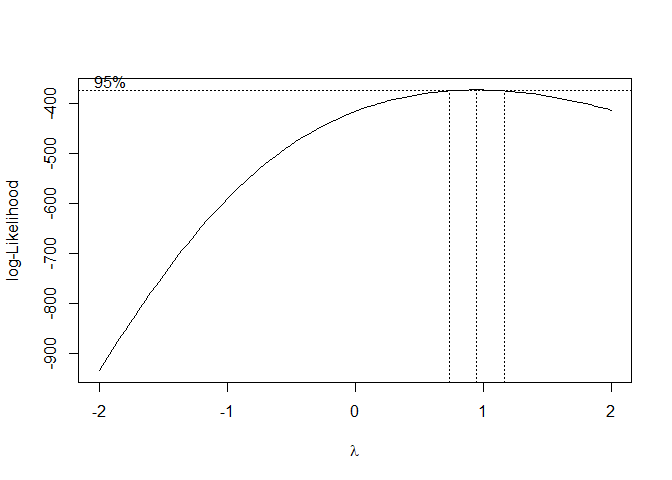
\includegraphics{proj_draft-1-_files/figure-latex/unnamed-chunk-10-1.pdf}

\begin{Shaded}
\begin{Highlighting}[]
\NormalTok{cv\_object}\SpecialCharTok{$}\NormalTok{lambda.min}
\end{Highlighting}
\end{Shaded}

\begin{verbatim}
## [1] 0.02511886
\end{verbatim}

\begin{Shaded}
\begin{Highlighting}[]
\NormalTok{fit\_bestcv }\OtherTok{\textless{}{-}} \FunctionTok{glmnet}\NormalTok{(}\FunctionTok{as.matrix}\NormalTok{(data\_train[,}\SpecialCharTok{{-}}\DecValTok{1}\NormalTok{]), data\_train}\SpecialCharTok{$}\NormalTok{bodyfat\_brozek, }\AttributeTok{lambda =}\NormalTok{ cv\_object}\SpecialCharTok{$}\NormalTok{lambda.min)}
\NormalTok{best\_lambda }\OtherTok{=}\NormalTok{ cv\_object}\SpecialCharTok{$}\NormalTok{lambda.min}
\FunctionTok{coef}\NormalTok{(fit\_bestcv)}
\end{Highlighting}
\end{Shaded}

\begin{verbatim}
## 14 x 1 sparse Matrix of class "dgCMatrix"
##                      s0
## (Intercept) -2.66318546
## age          0.06305549
## weight      -0.03981678
## height       .         
## neck        -0.35748584
## chest       -0.11450449
## abdomen      0.88564322
## hip         -0.19777927
## thigh        0.22445962
## knee        -0.18799617
## ankle        0.04664407
## bicep        0.07792838
## forearm      0.61660889
## wrist       -2.13035975
\end{verbatim}

\begin{Shaded}
\begin{Highlighting}[]
\NormalTok{lasso\_predict\_train }\OtherTok{=} \FunctionTok{predict}\NormalTok{(fit\_bestcv, }\AttributeTok{s =}\NormalTok{ best\_lambda, }\AttributeTok{newx =}\NormalTok{ X.train)}
\NormalTok{lasso\_predict\_test }\OtherTok{=} \FunctionTok{predict}\NormalTok{(fit\_bestcv, }\AttributeTok{s =}\NormalTok{ best\_lambda, }\AttributeTok{newx =}\NormalTok{ X.test)}
\NormalTok{RMSE\_LASSO }\OtherTok{=} \FunctionTok{sqrt}\NormalTok{(}\FunctionTok{mean}\NormalTok{((Y.test}\SpecialCharTok{{-}}\NormalTok{lasso\_predict\_test)}\SpecialCharTok{\^{}}\DecValTok{2}\NormalTok{))}
\NormalTok{SSE\_LASSO }\OtherTok{=} \FunctionTok{sum}\NormalTok{((Y.train }\SpecialCharTok{{-}}\NormalTok{ lasso\_predict\_train )}\SpecialCharTok{\^{}}\DecValTok{2}\NormalTok{)}
\NormalTok{SSTO\_LASSO }\OtherTok{=} \FunctionTok{sum}\NormalTok{((Y.train }\SpecialCharTok{{-}} \FunctionTok{mean}\NormalTok{(Y.train))}\SpecialCharTok{\^{}}\DecValTok{2}\NormalTok{)}
\NormalTok{n }\OtherTok{=} \FunctionTok{nrow}\NormalTok{(data\_train)}
\NormalTok{p }\OtherTok{=} \DecValTok{12}
\NormalTok{adj\_Rsquared\_LASSO\_trained }\OtherTok{=} \DecValTok{1} \SpecialCharTok{{-}}\NormalTok{ (SSE\_LASSO}\SpecialCharTok{/}\NormalTok{SSTO\_LASSO)}\SpecialCharTok{*}\NormalTok{((n}\DecValTok{{-}1}\NormalTok{)}\SpecialCharTok{/}\NormalTok{(n}\SpecialCharTok{{-}}\NormalTok{p}\DecValTok{{-}1}\NormalTok{))}
\NormalTok{adj\_Rsquared\_LASSO\_trained}
\end{Highlighting}
\end{Shaded}

\begin{verbatim}
## [1] 0.7439698
\end{verbatim}

\begin{Shaded}
\begin{Highlighting}[]
\NormalTok{RMSE\_LASSO}
\end{Highlighting}
\end{Shaded}

\begin{verbatim}
## [1] 4.578159
\end{verbatim}

\begin{Shaded}
\begin{Highlighting}[]
\FunctionTok{set.seed}\NormalTok{(}\DecValTok{100}\NormalTok{)}


\NormalTok{lambda\_seq }\OtherTok{\textless{}{-}} \DecValTok{10}\SpecialCharTok{\^{}}\FunctionTok{seq}\NormalTok{(}\SpecialCharTok{{-}}\DecValTok{3}\NormalTok{, }\DecValTok{0}\NormalTok{, }\AttributeTok{by =}\NormalTok{ .}\DecValTok{1}\NormalTok{)}
\NormalTok{cv\_object }\OtherTok{\textless{}{-}} \FunctionTok{cv.glmnet}\NormalTok{(}\FunctionTok{as.matrix}\NormalTok{(bd\_df[,}\SpecialCharTok{{-}}\DecValTok{1}\NormalTok{]), bd\_df}\SpecialCharTok{$}\NormalTok{bodyfat\_brozek, }\AttributeTok{lambda =}\NormalTok{ lambda\_seq, }
\AttributeTok{nfolds =} \DecValTok{5}\NormalTok{)}
\NormalTok{cv\_object}
\end{Highlighting}
\end{Shaded}

\begin{verbatim}
## 
## Call:  cv.glmnet(x = as.matrix(bd_df[, -1]), y = bd_df$bodyfat_brozek,      lambda = lambda_seq, nfolds = 5) 
## 
## Measure: Mean-Squared Error 
## 
##     Lambda Index Measure    SE Nonzero
## min 0.1259    10   17.91 1.518       7
## 1se 0.5012     4   19.09 1.800       4
\end{verbatim}

\begin{Shaded}
\begin{Highlighting}[]
\FunctionTok{tibble}\NormalTok{(}\AttributeTok{lambda =}\NormalTok{ cv\_object}\SpecialCharTok{$}\NormalTok{lambda,}
\AttributeTok{mean\_cv\_error =}\NormalTok{ cv\_object}\SpecialCharTok{$}\NormalTok{cvm) }\SpecialCharTok{\%\textgreater{}\%}
\FunctionTok{ggplot}\NormalTok{(}\FunctionTok{aes}\NormalTok{(}\AttributeTok{x =}\NormalTok{ lambda, }\AttributeTok{y =} 
\NormalTok{mean\_cv\_error)) }\SpecialCharTok{+}
\FunctionTok{geom\_point}\NormalTok{()}
\end{Highlighting}
\end{Shaded}

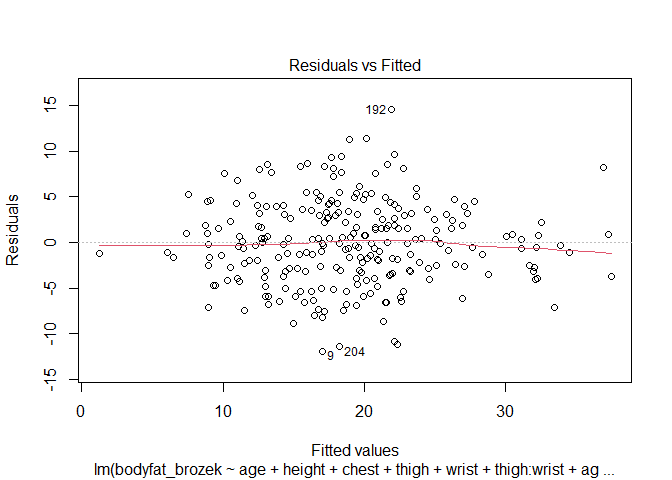
\includegraphics{proj_draft-1-_files/figure-latex/unnamed-chunk-13-1.pdf}

\begin{Shaded}
\begin{Highlighting}[]
\NormalTok{cv\_object}\SpecialCharTok{$}\NormalTok{lambda.min}
\end{Highlighting}
\end{Shaded}

\begin{verbatim}
## [1] 0.1258925
\end{verbatim}

\begin{Shaded}
\begin{Highlighting}[]
\NormalTok{fit\_bestcv }\OtherTok{\textless{}{-}} \FunctionTok{glmnet}\NormalTok{(}\FunctionTok{as.matrix}\NormalTok{(bd\_df[,}\SpecialCharTok{{-}}\DecValTok{1}\NormalTok{]), bd\_df}\SpecialCharTok{$}\NormalTok{bodyfat\_brozek, }\AttributeTok{lambda =}\NormalTok{ cv\_object}\SpecialCharTok{$}\NormalTok{lambda.min)}
\NormalTok{best\_lambda }\OtherTok{=}\NormalTok{ cv\_object}\SpecialCharTok{$}\NormalTok{lambda.min}
\FunctionTok{coef}\NormalTok{(fit\_bestcv)}
\end{Highlighting}
\end{Shaded}

\begin{verbatim}
## 14 x 1 sparse Matrix of class "dgCMatrix"
##                        s0
## (Intercept)  3.3119530764
## age          0.0543537828
## weight       .           
## height      -0.2643337237
## neck        -0.3128557105
## chest        .           
## abdomen      0.6705061093
## hip         -0.0006719874
## thigh        .           
## knee         .           
## ankle        .           
## bicep        .           
## forearm      0.2637571652
## wrist       -1.4190640738
\end{verbatim}

\begin{Shaded}
\begin{Highlighting}[]
\CommentTok{\# Use 5{-}fold validation and create the training sets}
\NormalTok{train }\OtherTok{=} \FunctionTok{trainControl}\NormalTok{(}\AttributeTok{method =} \StringTok{"cv"}\NormalTok{, }\AttributeTok{number =} \DecValTok{5}\NormalTok{)}
\CommentTok{\# Fit the variables model }
\NormalTok{model\_caret }\OtherTok{=} \FunctionTok{train}\NormalTok{(bodyfat\_brozek }\SpecialCharTok{\textasciitilde{}}\NormalTok{ age }\SpecialCharTok{+}\NormalTok{  height }\SpecialCharTok{+}\NormalTok{ neck }\SpecialCharTok{+}\NormalTok{ abdomen }\SpecialCharTok{+}\NormalTok{hip}\SpecialCharTok{+}\NormalTok{forearm}\SpecialCharTok{+}\NormalTok{wrist,}
\AttributeTok{data =}\NormalTok{ bd\_df,}
\AttributeTok{trControl =}\NormalTok{ train,}
\AttributeTok{method =} \StringTok{\textquotesingle{}lm\textquotesingle{}}\NormalTok{,}
\AttributeTok{na.action =}\NormalTok{ na.pass)}
\NormalTok{model\_caret}
\end{Highlighting}
\end{Shaded}

\begin{verbatim}
## Linear Regression 
## 
## 251 samples
##   7 predictor
## 
## No pre-processing
## Resampling: Cross-Validated (5 fold) 
## Summary of sample sizes: 199, 201, 202, 201, 201 
## Resampling results:
## 
##   RMSE     Rsquared   MAE     
##   4.10807  0.7331927  3.303071
## 
## Tuning parameter 'intercept' was held constant at a value of TRUE
\end{verbatim}

\end{document}
